%!TEX program = xelatex
%!TEX spellcheck = en_GB
\documentclass[final]{report}
% Include all project wide packages here.
%\usepackage{fullpage}
\usepackage[a4paper,margin=2.5cm,top=2cm]{geometry}
\usepackage{polyglossia}
\setmainlanguage{english}
\usepackage{csquotes}
\usepackage{graphicx}
\usepackage{pdfpages}
\usepackage{caption}
\usepackage[list=true]{subcaption}
\usepackage{float}
\usepackage{standalone}
\usepackage{import}
\usepackage{tocloft}
\usepackage{wrapfig}
\usepackage{authblk}
\usepackage{array}
\usepackage{booktabs}
\usepackage[title,titletoc]{appendix}
\usepackage{fontspec}
\usepackage{pgfplots}
\usepackage{tikz}
\usepackage[binary-units=true]{siunitx}
\usepackage{units}
\usepackage{amsmath}
\usepackage{mathtools}
\usepackage{unicode-math}
\usepackage{rotating}
\usepackage{titlesec}
\usepackage{titletoc}
\usepackage{blindtext}
\usepackage{color}
\usepackage{enumitem}
\usepackage{tabularx}
\usepackage{titling}
\usepackage[%
siunitx,
fulldiodes,
europeanvoltages,
europeancurrents,
europeanresistors,
americaninductors,
smartlabels]{circuitikz}

\newcommand{\matlab}{{\textsc{matlab }}}

\usetikzlibrary{calc}
\usetikzlibrary{positioning}
\usetikzlibrary{automata}
\usetikzlibrary{arrows.meta}

\tikzstyle{every state}=[fill=tu-cyan,align=center,draw=black,line width=1pt,node distance=3cm,minimum width = 1.8cm]%for FSMs casper
\tikzstyle{every initial by arrow}=[initial text={Reset}]
\newcommand{\setpathasarrows}{\tikzstyle{every path}=[auto,line width=1.5pt,line cap=round,line join=round]}

\pgfplotsset{compat=newest}
\pgfplotsset{plot coordinates/math parser=false}
\usetikzlibrary{plotmarks}
\usepgfplotslibrary{patchplots}
\newlength\figureheight
\newlength\figurewidth

\tikzset{every axis/.style={xticklabel style={align=right}}}

\usepackage[
%backend=bibtex,
backend=biber,
	texencoding=utf8,
bibencoding=utf8,
style=numeric,
citestyle=numeric,
    sortlocale=en_US,
    language=auto,
    backref=true,
    abbreviate=false,
    date=edtf,
    seconds=true
]{biblatex}


\usepackage{listings}
\newcommand{\includecode}[4][c]{\lstinputlisting[caption=#2, escapechar=, style=#1,label=#4]{#3}}
\newcommand{\superscript}[1]{\ensuremath{^{\textrm{#1}}}}
\newcommand{\subscript}[1]{\ensuremath{_{\textrm{#1}}}}


\newcommand{\chapternumber}{\thechapter}
\renewcommand{\appendixname}{Appendix}
\renewcommand{\appendixtocname}{Appendices}
\renewcommand{\appendixpagename}{Appendices}


\setlist[enumerate]{labelsep=*, leftmargin=1.5pc}
\setlist[enumerate,1]{label=\arabic*., ref=\arabic*}
\setlist[enumerate,2]{label=\arabic*.,ref=\theenumi.\arabic*}
\setlist[enumerate,3]{label=\arabic*., ref=\theenumii.\arabic*}

%\setcounter{chapter}{-1} %start chapter numbers with 0

\usepackage{xr-hyper}
\usepackage[hidelinks]{hyperref} %<--------ALTIJD ALS LAATSTE
\usepackage[nameinlink,noabbrev,capitalise]{cleveref} %<------- Clever Ref moet na hyperref
\crefname{app}{Appendix}{Appendices}
%\renewcommand{\familydefault}{\sfdefault}


\setmainfont{Myriad Pro}[Ligatures={Common,TeX}]
\setmathfont{Asana Math}
\setmonofont[Scale=0.9]{Lucida Console}
\newfontfamily\headingfont{Minion Pro}[Ligatures={Common,TeX}]


%Design colors
\definecolor{accent1}{RGB}{0,100,200}
\definecolor{accent2}{RGB}{0,50,100}
\definecolor{tu-cyan}{RGB}{0,166,214}

\newcommand{\hsp}{\hspace{20pt}}
\titleformat{\chapter}[hang]{\Huge\headingfont}{\chapternumber\hsp\textcolor{accent2}{|}\hsp}{0pt}{\Huge\headingfont}

\titleformat{name=\chapter,numberless}[hang]{\Huge\headingfont}{\hsp\textcolor{accent2}{|}\hsp}{0pt}{\Huge\headingfont}

\titleformat{\section}[block]{\LARGE\headingfont}{\arabic{chapter}.\arabic{section}}{0.4em}{}
\titleformat{\subsection}[block]{\Large\headingfont}{\arabic{chapter}.\arabic{section}.\arabic{subsection}}{0.4em}{}
\titleformat{\subsubsection}[block]{\large\headingfont}{\arabic{chapter}.\arabic{section}.\arabic{subsection}.\arabic{subsubsection}}{0.4em}{}
\renewcommand{\arraystretch}{1.2}
\renewcommand{\baselinestretch}{1.25} 

\renewcommand\cfttoctitlefont{\headingfont\Huge}
\renewcommand\cftloftitlefont{\headingfont\Huge}
\renewcommand\cftlottitlefont{\headingfont\Huge}
\setcounter{lofdepth}{2}
\setcounter{lotdepth}{2}


\setlength{\parindent}{0pt}
\setlength{\parskip}{1em}


%SIuntix settings:
%default: 0V to 10V
%custom: 0 - 10V
\sisetup{range-phrase=--}
\sisetup{range-units=single}
\DeclareSIUnit\years{years}

%For code listings
\definecolor{black}{rgb}{0,0,0}
\definecolor{browntags}{rgb}{0.65,0.1,0.1}
\definecolor{bluestrings}{rgb}{0,0,1}
\definecolor{graycomments}{rgb}{0.4,0.4,0.4}
\definecolor{redkeywords}{rgb}{1,0,0}
\definecolor{bluekeywords}{rgb}{0.13,0.13,0.8}
\definecolor{greencomments}{rgb}{0,0.5,0}
\definecolor{redstrings}{rgb}{0.9,0,0}
\definecolor{purpleidentifiers}{rgb}{0.01,0,0.01}


\lstdefinestyle{csharp}{
language=[Sharp]C,
showspaces=false,
showtabs=false,
breaklines=true,
showstringspaces=false,
breakatwhitespace=true,
escapeinside={(*@}{@*)},
columns=fullflexible,
commentstyle=\color{greencomments},
keywordstyle=\color{bluekeywords}\bfseries,
stringstyle=\color{redstrings},
identifierstyle=\color{purpleidentifiers},
basicstyle=\ttfamily\small}

\lstdefinestyle{c}{
language=C,
showspaces=false,
showtabs=false,
breaklines=true,
showstringspaces=false,
breakatwhitespace=true,
escapeinside={(*@}{@*)},
columns=fullflexible,
commentstyle=\color{greencomments},
keywordstyle=\color{bluekeywords}\bfseries,
stringstyle=\color{redstrings},
identifierstyle=\color{purpleidentifiers},
}

\lstdefinestyle{matlab}{
language=Matlab,
showspaces=false,
showtabs=false,
breaklines=true,
showstringspaces=false,
breakatwhitespace=true,
escapeinside={(*@}{@*)},
columns=fullflexible,
commentstyle=\color{greencomments},
keywordstyle=\color{bluekeywords}\bfseries,
stringstyle=\color{redstrings},
identifierstyle=\color{purpleidentifiers}
}

\lstdefinestyle{vhdl}{
language=VHDL,
showspaces=false,
showtabs=false,
breaklines=true,
showstringspaces=false,
breakatwhitespace=true,
escapeinside={(*@}{@*)},
columns=fullflexible,
commentstyle=\color{greencomments},
keywordstyle=\color{bluekeywords}\bfseries,
stringstyle=\color{redstrings},
identifierstyle=\color{purpleidentifiers}
}

\lstdefinestyle{xaml}{
language=XML,
showspaces=false,
showtabs=false,
breaklines=true,
showstringspaces=false,
breakatwhitespace=true,
escapeinside={(*@}{@*)},
columns=fullflexible,
commentstyle=\color{greencomments},
keywordstyle=\color{redkeywords},
stringstyle=\color{bluestrings},
tagstyle=\color{browntags},
morestring=[b]",
  morecomment=[s]{<?}{?>},
  morekeywords={xmlns,version,typex:AsyncRecords,x:Arguments,x:Boolean,x:Byte,x:Char,x:Class,x:ClassAttributes,x:ClassModifier,x:Code,x:ConnectionId,x:Decimal,x:Double,x:FactoryMethod,x:FieldModifier,x:Int16,x:Int32,x:Int64,x:Key,x:Members,x:Name,x:Object,x:Property,x:Shared,x:Single,x:String,x:Subclass,x:SynchronousMode,x:TimeSpan,x:TypeArguments,x:Uid,x:Uri,x:XData,Grid.Column,Grid.ColumnSpan,Click,ClipToBounds,Content,DropDownOpened,FontSize,Foreground,Header,Height,HorizontalAlignment,HorizontalContentAlignment,IsCancel,IsDefault,IsEnabled,IsSelected,Margin,MinHeight,MinWidth,Padding,SnapsToDevicePixels,Target,TextWrapping,Title,VerticalAlignment,VerticalContentAlignment,Width,WindowStartupLocation,Binding,Mode,OneWay,xmlns:x}
}

\lstdefinestyle{python}{
language=Python,
showspaces=false,
showtabs=false,
breaklines=true,
showstringspaces=false,
breakatwhitespace=true,
escapeinside={(*@}{@*)},
columns=fullflexible,
commentstyle=\color{greencomments},
keywordstyle=\color{bluekeywords}\bfseries,
stringstyle=\color{redstrings},
identifierstyle=\color{purpleidentifiers},
}

%defaults
\lstset{
basicstyle=\ttfamily\scriptsize ,
extendedchars=false,
numbers=left,
numberstyle=\ttfamily\tiny,
stepnumber=1,
tabsize=4,
numbersep=5pt
}
\addbibresource{../../.library/bibliography.bib}

\begin{document}
\chapter{Uncompleted Results}
\label{ch:Uncompleted Results}

This chapter contains work that is uncompleted that was intended to be part of the project, but for several possible reasons was not included or not finished. That could be not enough time, unsuited tools or we couldn't get it to work. So if one wants to follow up on the project, these are several topics which could be further developed:

\begin{enumerate}
	\item Speech recognition
	\item Training
	\item Classifier
	\item Game metadata
	\item Twitch API fix
\end{enumerate}

\section{SpeechRecognition}
Originally we wanted to analyse the interaction between the streamer and the users, so we needed data from the streamer.
The downloaded audio was used with the python library SpeechRecognition. %https://pypi.python.org/pypi/SpeechRecognition/%.
Different speech recognition toolkits were looked into:
\begin{enumerate}
\item Python speech recognition 3.7.1 which includes CMU Sphinx as speech recognition software. It is very slow as the processing must happen in real-time.
\item Dragon Speech Recognition Software, which is a professional software package. However it has high price which makes it not viable for our project.
\item Google Cloud Speech API, google has a free tool that can be used for speech recognition. It is however very slow like all other tools and does not return usable text.
\end{enumerate}

All the tools used work in real-time, so this means they are all very slow (each second of audio takes 1 second to process). Likewise none of them returned usable data that doesn't contain a significant amount of errors.
This is expected as speech recognition is still not at the required level to properly gather reliable data, moreover music is usually played on stream and together with game sounds this interferes significantly with the speech recognition.
We conclude that speech recognition on a massive dataset is still not a viable option.
In the near future when services are cheaper and the recognition technology is more advanced it could become interesting to look into this.

\section{Training}
To analyse the chat data, we had to gather a training set in which the chat is rated based on their toxicity.
We converted the compressed pickle file to a chat log from the MLG channel to an SQL insert statement to store the chat into a MySQL database.
A website implemented in JavaScript and PHP showed this chat and we manually rated each chat message with a 1 to 5 (1 being non-toxic, 5 being very toxic). The final training set is also filtered on words that are shorter than 3 letters to remove even more noise. Below the web page where the data can be trained is shown in \ref{fig:rating}.

\begin{figure}[h]
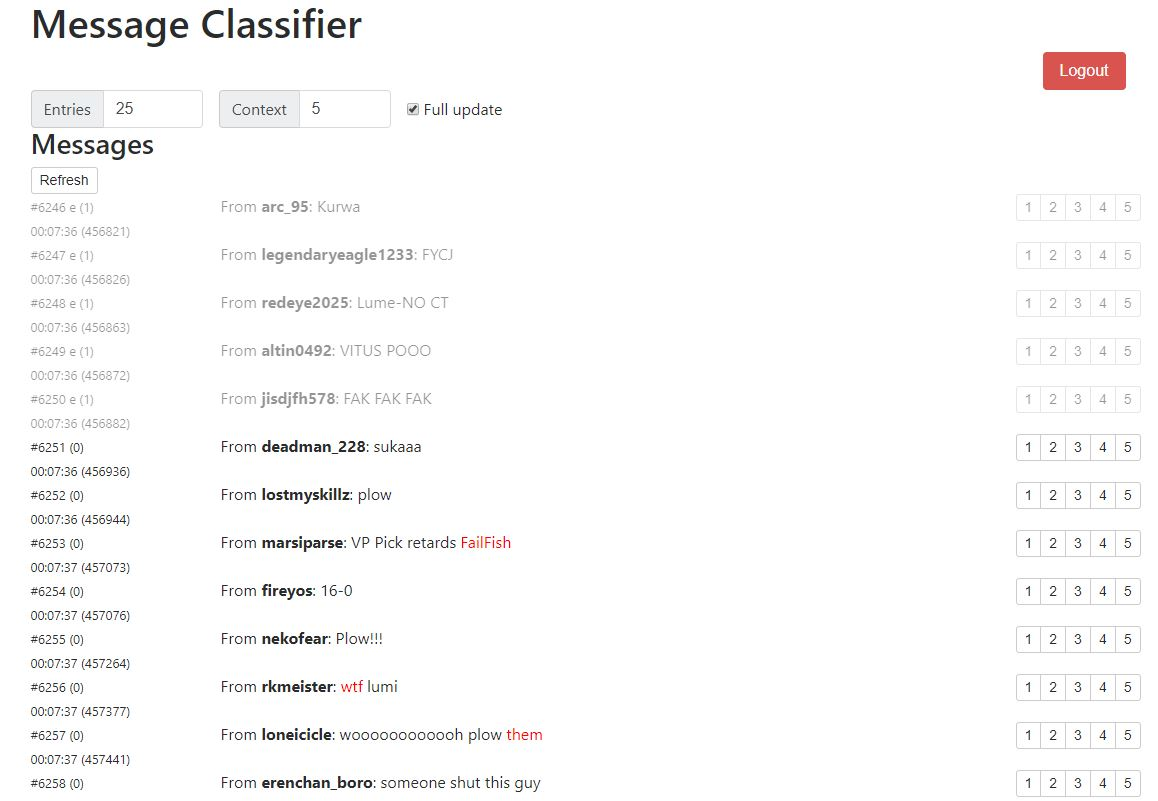
\includegraphics[scale=0.5]{rating}
\caption{Web page to train our dataset}
\label{fig:rating}
\end{figure}

On the far left the message number and the timestamp of the message is shown, together with how often the message has been rated before (between the brackets). In the middle the user (bold) and the message sent by the user can be seen to determine the rating. On the far right are the rating options, with 1 being non toxic and 5 very toxic.

\section{Classifier}
%NLTK

%From results, about the classifier
After the training set is complete and present in the database it can be used to classify other data. The classifier downloads a sub set of the manually classified data, then extracts word based features and trains a classifier.
The problem was in the initial distribution of all the classes for the classifier.
There are way too many messages rated 1 (non-toxic). Thus the output of the classified was mostly 1.000 (float). Other classifiers that could be used instead of the current Python NLTK are:

\begin{enumerate}
	\item \textbf{VADER Sentiment Analysis}, Valence Aware Dictionary and sEntiment Reasoner. This is a lexicon and rule-based sentiment analysis tool that is specifically attuned to sentiments expressed in social media, and works well on texts from other domains \cite{vader}.
	\item \textbf{Naive Bayes}, a text classifier based on Naive Bayes. Which are methods of supervised learning algorithms based on applying Bayes' theorem with the "naive" assumption of independence between every pair of features \cite{naivebayes}.
	\item \textbf{MaxEnt}, Maximum Entropy Classifiers. This is a classifier model that is based on the maximum entropy modeling framework. This framework considers all of the probability distributions that are empirically consistent with the training data; and chooses the distribution with the highest entropy \cite{maxent}.
\end{enumerate}

The idea was that the results would give an average degree of toxicity for certain streamers to compare, but also users individually per channel viewed. Based on those results different viewers could also be compared in different channels to see how the toxicity in a channel affects the viewers. So in other words if the toxicity in twitch streams is also contagious.

\section{Game Metadata}

If somehow the game metadata of what is happening in game with timestamps could be obtained it would be highly valuable to give better insight in why the chat responds in certain ways. Speech recognition was one of the options to achieve this, but will always give results with high noise in the data. If this metadata could be obtained from the game itself it would contain no noise.

\section{Twitch API}

Unfortunately the current Twitch API does not always return what is expected. For example when trying to download all the videos of the company behind League of Legends, Riotgames, from Twitch, it returns only a fraction of the expected videos which are highly outdated and currently of no use. As this is the responsibility of Twitch there is currently little that can be done about this, in the future when Twitch could have updated their API the video download script might work more optimal.


\end{document}